\chapter{Getting Started with plapack}
\label{chapter:getstart}


In this chapter, we present the basic calls provided by
plapack to initialize the environment, create a template\footnote{
Notice, our use of the word template should not be confused with
the use of templates in C++.}
(description) for the distribution of vectors and matrices,
and create linear algebra objects that describe the
distributed vectors and matrices.


%%%%%%%%%%%%%%%%%%%%%%%%%%%%%%%%%%%%%%%%%%%%%%%%%%
\section{Initializing and Finalizing plapack}

Before using the plapack, the environment must be initialized with a call to
\begin{FlaSpec}
\begin{verbatim}
PLA_Init( )
\end{verbatim}
\purpose{
Initialize plapack environment.
} 
\end{FlaSpec}
If no more plapack calls are to be made, the environment is exited by calling
\begin{FlaSpec}
\begin{verbatim}
PLA_Finalize( )
\end{verbatim}
\purpose{
Finalize plapack environment.
} 
\end{FlaSpec}
Since an application may wish to use a number of packages,
each of which themselves may use plapack, we provide an inquiry
routine to check if plapack has already been initialized with
\begin{FlaSpec}
\begin{verbatim}
PLA_Bool PLA_Initialized( )
\end{verbatim}
\purpose{
Check if plapack is initialized.
}
\parameter{return}{indicates whether plapack is already initialized} 
\end{FlaSpec}
The output argument equals {\tt FALSE}(= 0) if plapack has not been 
initialized and {\tt TRUE}($\neq$ 0) if it has.


%%%%%%%%%%%%%%%%%%%%%%%%%%%%%%%%%%%%%%%%%%%%%%%%%%
\section{Distribution Templates}

Rather than describing the distribution of each individual
vector and matrix directly, the plapack infrastructure requires
the distribution of (imaginary) {\em template} vectors and matrices to
be described. Vector and matrix distribution is
given by indicating alignment with respect to these template vectors and matrices.

Imagine an infinite length column vector $ t $, which is partitioned as
\[
t = \left( \begin{array}{c}
t_0 \\ \hline
t_1 \\ \hline
t_2 \\ \hline
\vdots
\end{array}
\right)
\]
with all $ t_i $ of uniform length $ n_b $, the column vector
distribution blocking size (see Figure~\ref{fig:vecalign}).
\begin{figure}[htbp]
\begin{center}
\begin{tabular}{ c c }
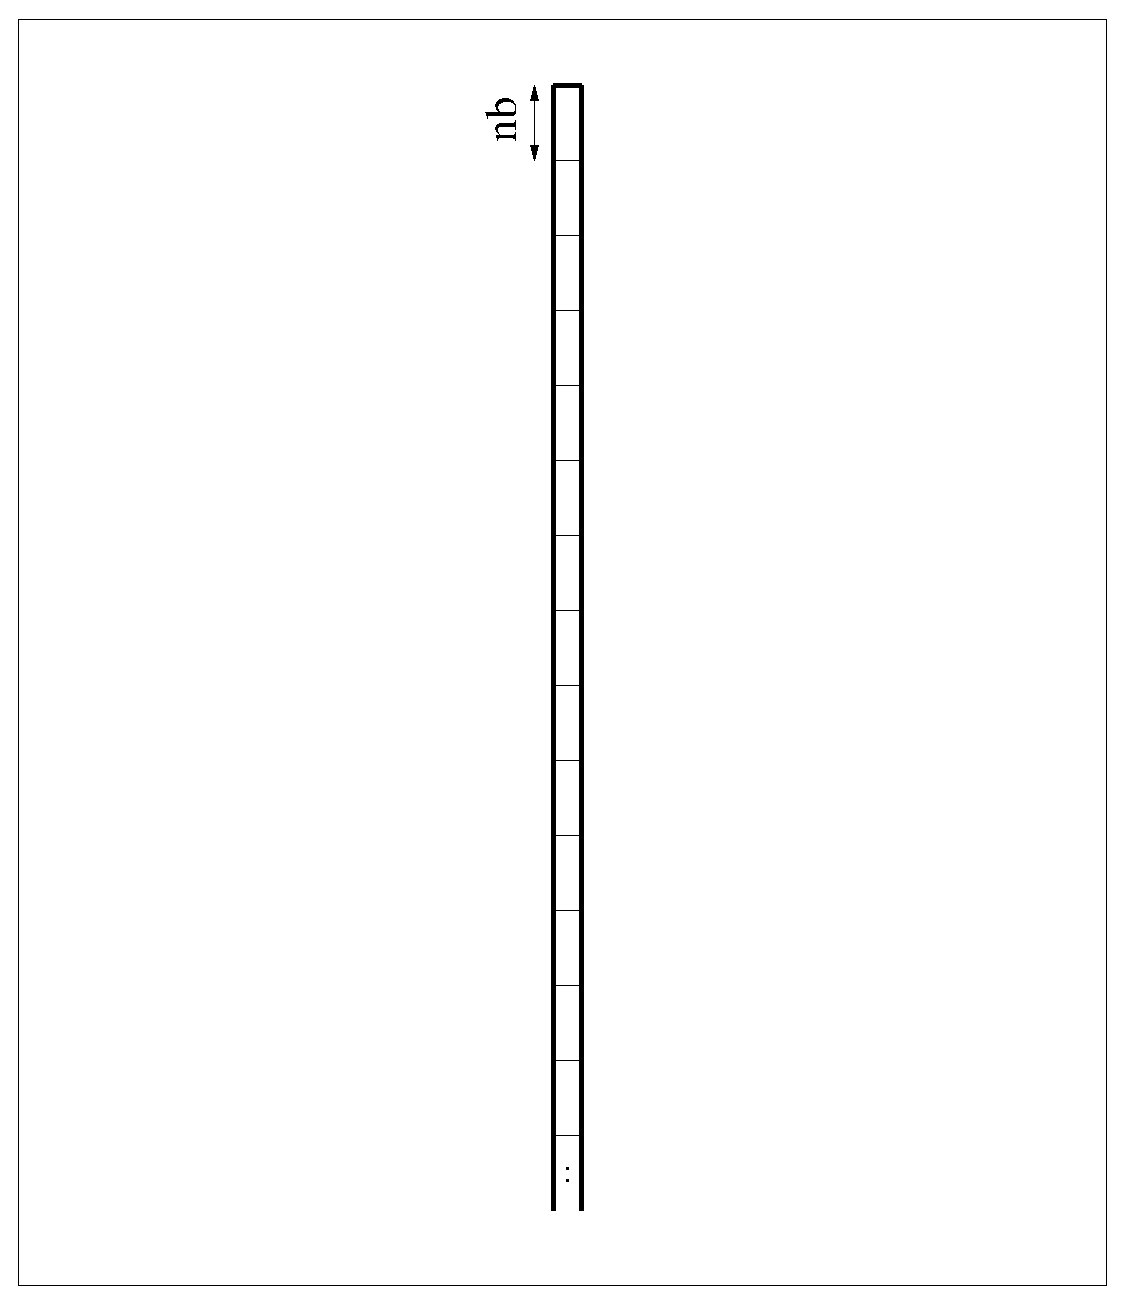
\includegraphics[height=2.75in,width=2.75in]{figures/vecttemp.eps} 
&
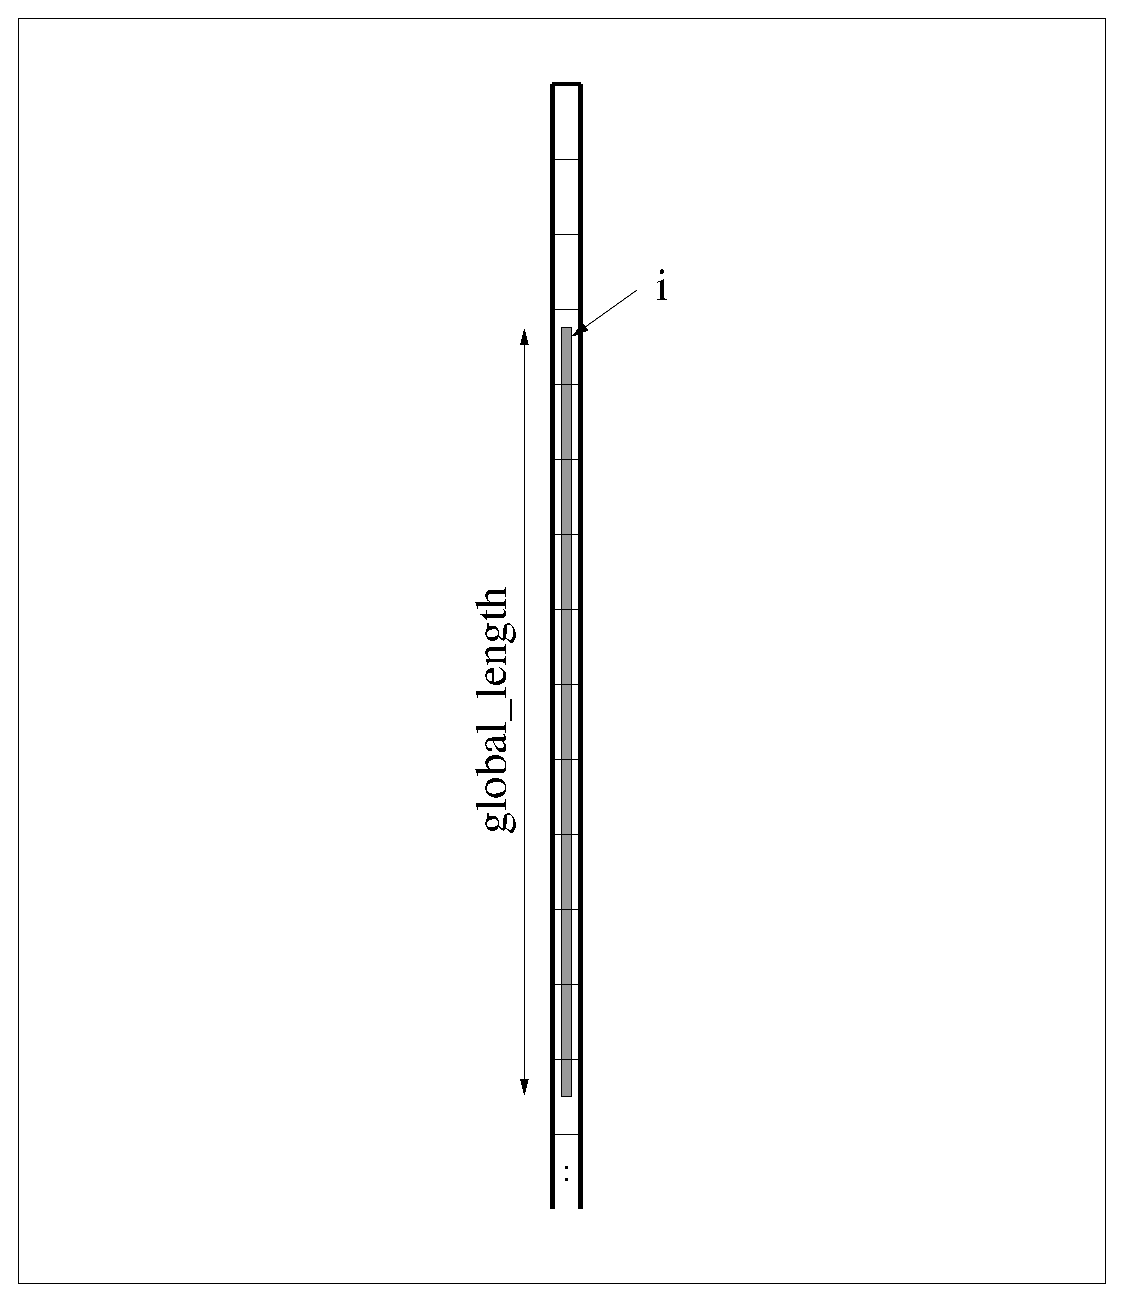
\includegraphics[height=2.75in,width=2.75in]{figures/vectalign.eps} 
\\
\multicolumn{2}{c}{
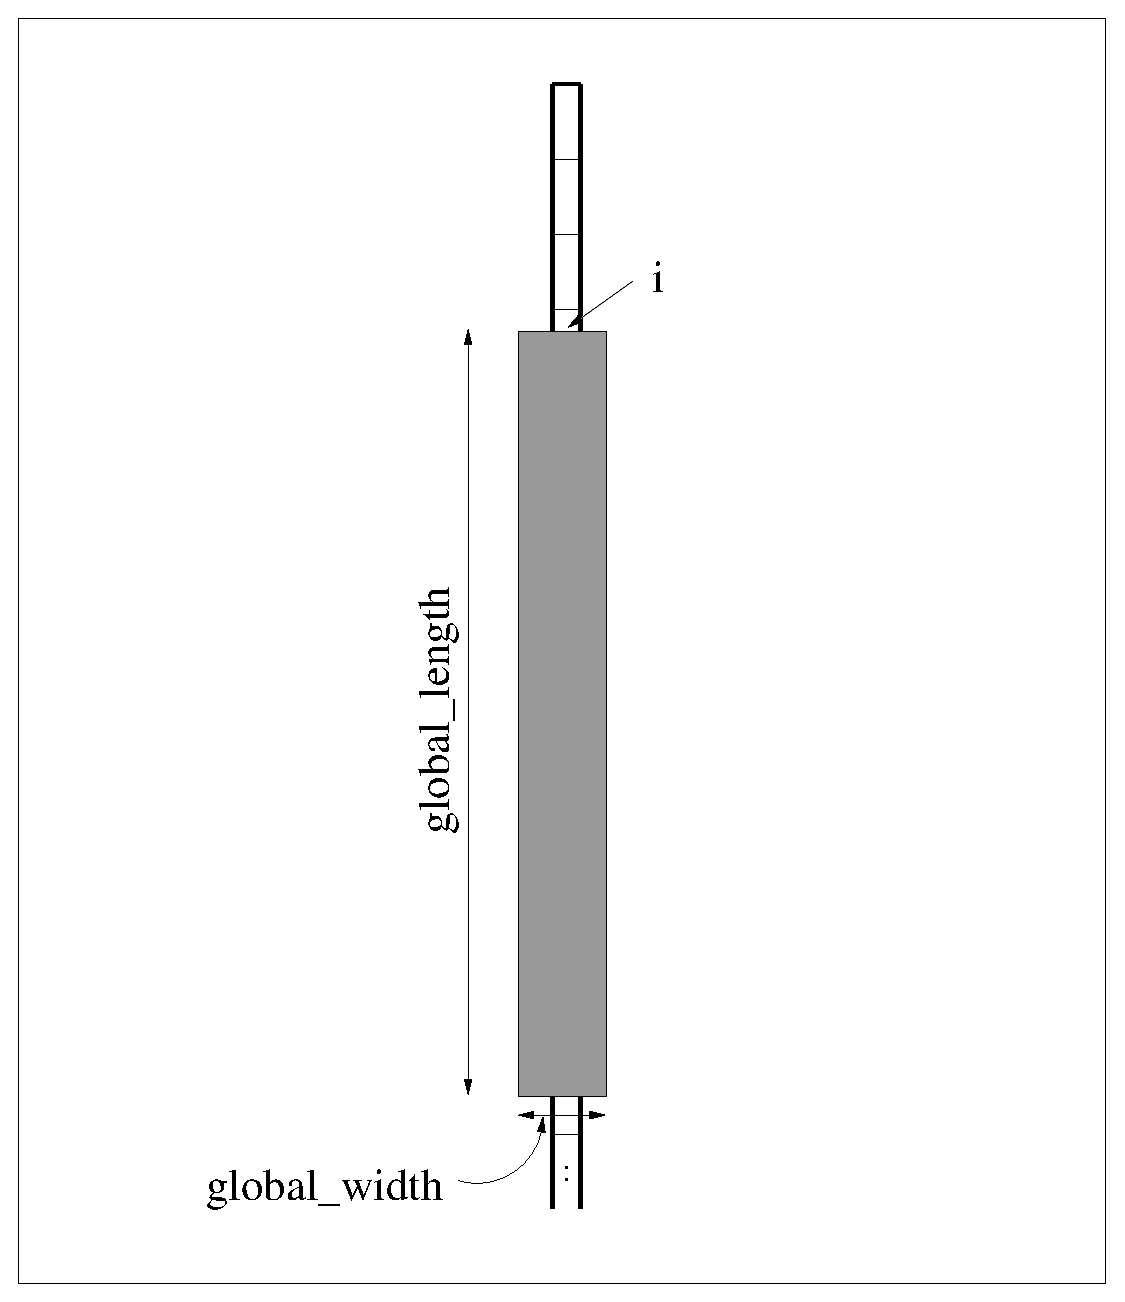
\includegraphics[height=2.75in,width=2.75in]{figures/mvectalign.eps}
}
\end{tabular}
\end{center}
\caption{Left: Template for column vector alignment.
Right: Column vector alignment to the template.
Bottom: Multivector alignment to the template.}
\label{fig:vecalign}
\end{figure}
Sub-vectors are assigned to the logical two dimensional
mesh corresponding to an MPI communicator
by wrapping in either row or column major order.
We will call this vector the {\bf template column vector}.

A distributed column vector is {\bf aligned} to this template column vector
by indicating the element of the template column vector with which
the first element of the column vector to be distributed is aligned,
as illustrated in Figure~\ref{fig:vecalign}.
The distribution of the elements of the column vector to be distributed
is then dictated by the distribution of corresponding elements
to the template column vector.
Thus if the first element of the column vector is aligned with
element $ i $ of the template column vector,
the $ j $th element of the column vector to be distributed is
assigned to the same node as the $ i+j $th element
of the template column vector.

The distribution of matrices is now induced by both template 
row and column vectors.
More specifically, let $ T $ be an infinite matrix,
partitioned as
\[
T = \left( \begin{array}{c | c | c | c}
T_{0,0} & T_{0,1} &  T_{0,2} & \cdots \\ \hline
T_{1,0} & T_{1,1} &  T_{1,2} & \cdots \\ \hline
T_{2,0} & T_{2,1} &  T_{2,2} & \cdots \\ \hline
\vdots &  \vdots  &  \vdots  &
\end{array}
\right)
\]
where $ T_{i,j} $ are $ m_b \times n_b $ sub-matrices.
Then this matrix is distributed to
nodes as induced by the template row and column vectors,
$ t^r$ and $ t^c $.
A given matrix to be distributed is now aligned to
this template by indicating the element of $ T $ with
which the top-left element of the matrix to be distributed
is aligned, as illustrated in  Figure~\ref{fig:matrixalign}.
\begin{figure}[htbp]
\begin{center}
\begin{tabular}{ c c }
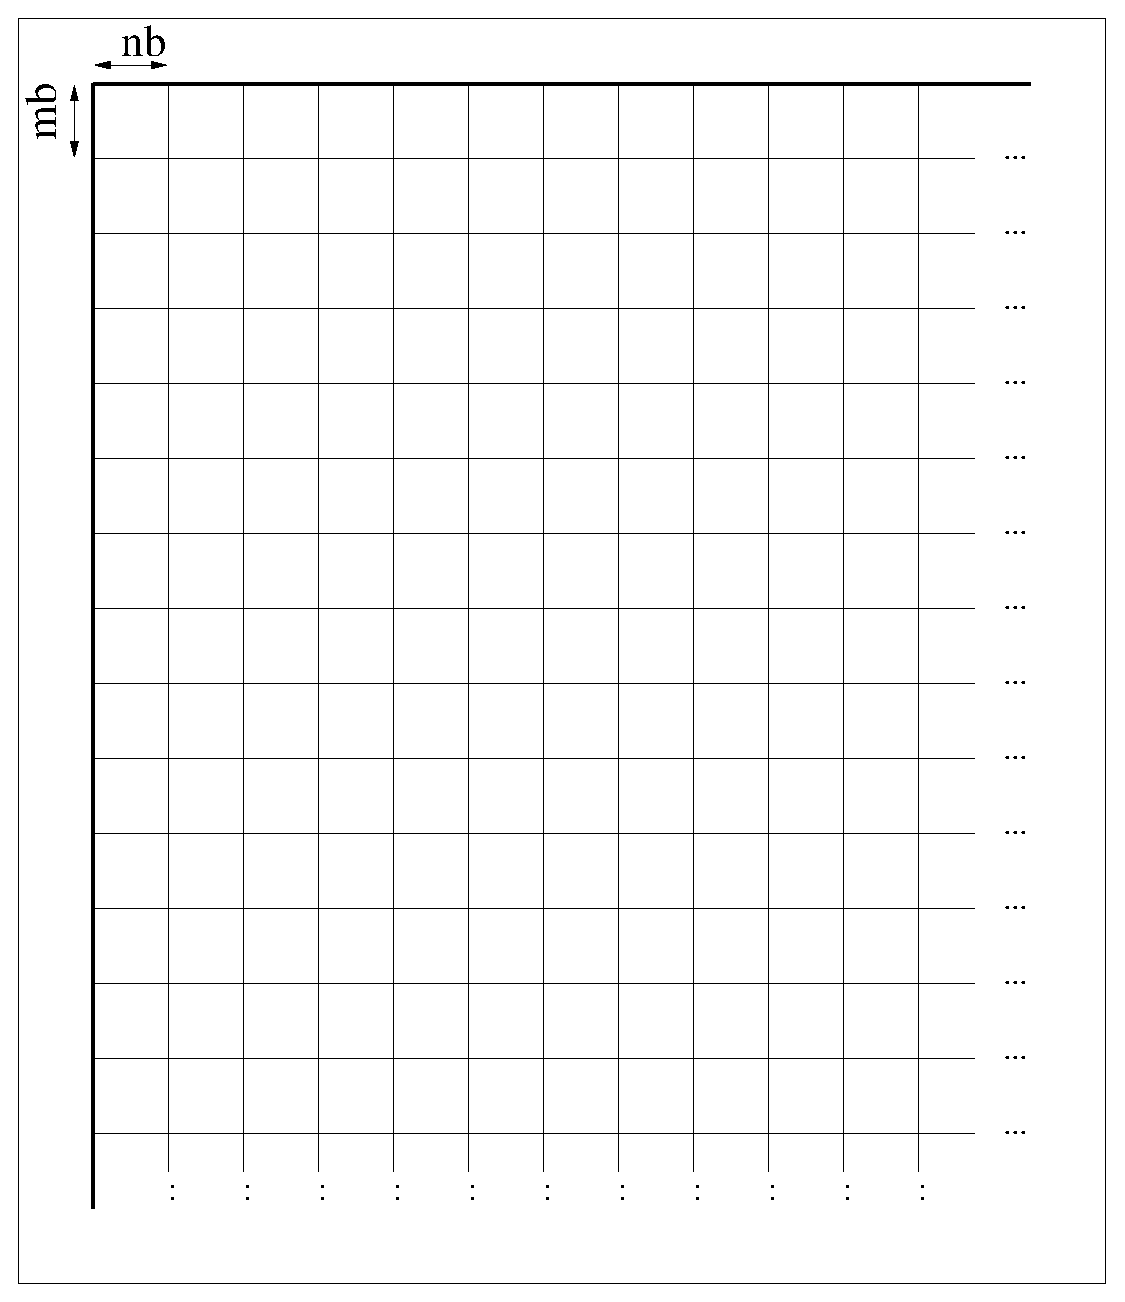
\includegraphics[height=2.75in,width=2.75in]{figures/template.eps}
&
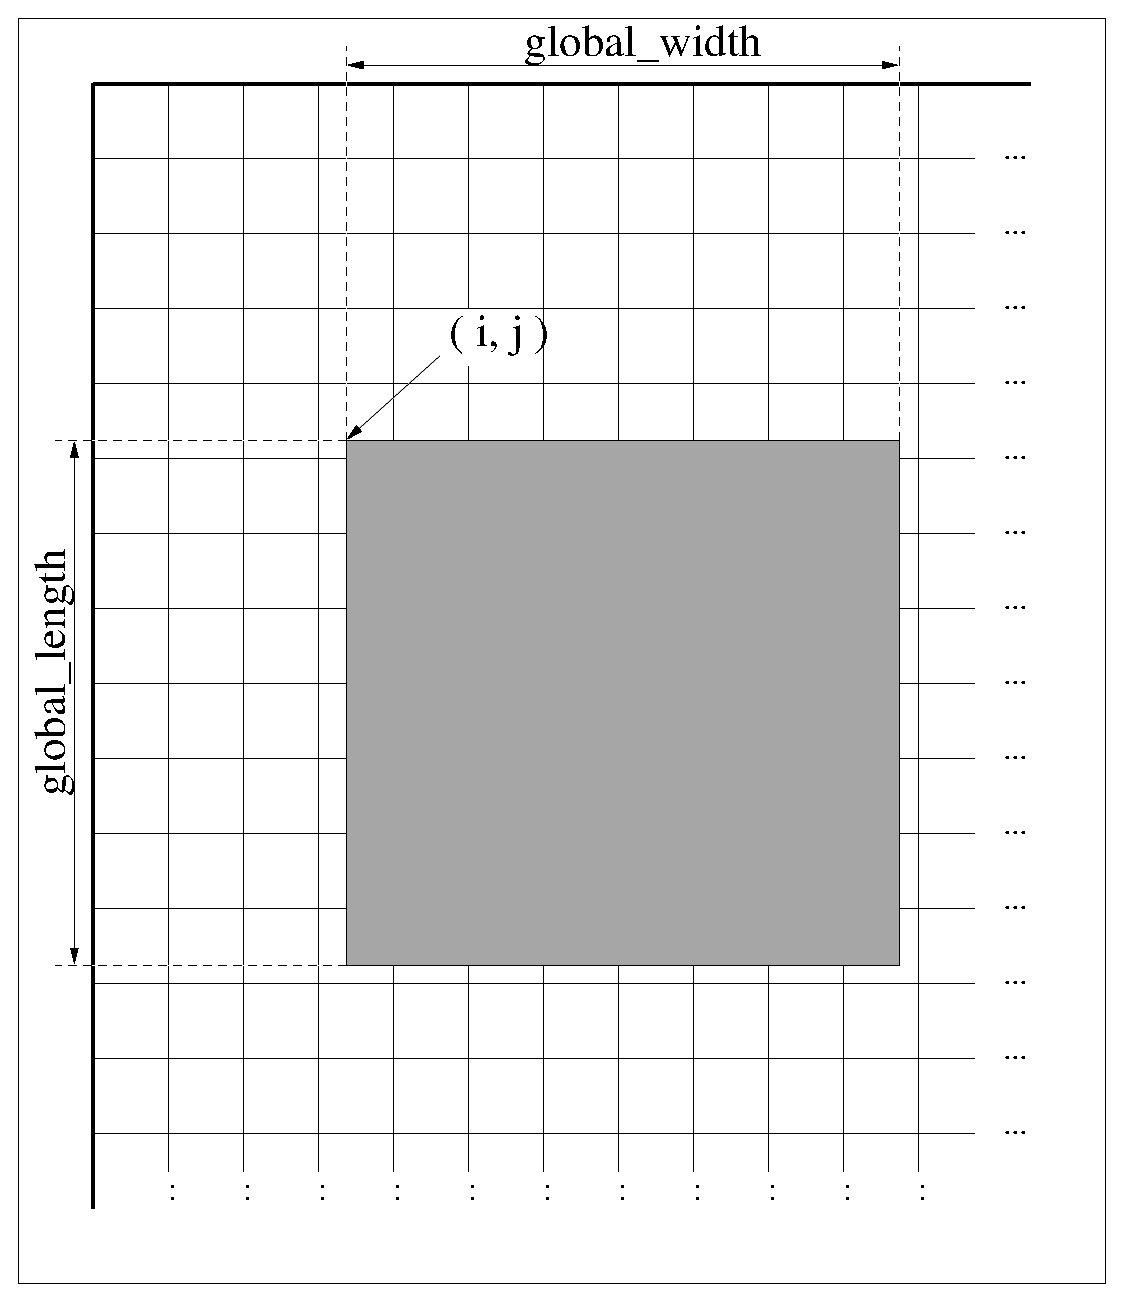
\includegraphics[height=2.75in,width=2.75in]{figures/align.eps}
\end{tabular}
\end{center}
\caption{Left: Template for matrix alignment.
Right: Matrix alignment to the template.}
\label{fig:matrixalign}
\end{figure}


\subsection{Template creation}

Initializing the template is accomplished with a call to the routine
\begin{FlaSpec}
\begin{verbatim}
PLA_Temp_create( MPI_Comm comm, int nprows, int npcols, 
                 int mb, PLA_Distr colDistr, 
                 int nb, PLA_Distr rowDistr, 
                 PLA_Temp *templ )
\end{verbatim}
\purpose{
Create template for vector and matrix distribution.
}
\parameter{\tt comm}{base communicator to be used by the template}
\parameter{\tt nprows}{number of rows to create 2D communicator}
\parameter{\tt npcols}{number of columns to create 2D communicator}
\parameter{\tt mb}{length of sub-vectors of template column vector}
\parameter{\tt colDistr}{direction for laying out column vector}
\parameter{\tt nb}{length of sub-vectors of template row vector}
\parameter{\tt rowDistr}{direction for laying out row vector}
\parameter{templ}{template for vector and matrix distribution} 
\end{FlaSpec}
Here the parameter {\tt comm} equals an MPI communicator specifying
the nodes to be used by the template.  The underlying system
generates a two-dimensional topology with the communicator with
the ratio given by {\tt nprows} $\times$ {\tt npcols} which 
does not have to be attainable: it is only a {\em suggestion}.
{\tt PLA\_Distr} for laying out the column and row directions can each be
either {\tt PLA\_ROW\_MAJOR} or {\tt PLA\_COL\_MAJOR}.

A predefined template {\tt PLA\_TEMP\_WORLD} is also provided to circumvent
the creation of templates.  {\tt PLA\_TEMP\_WORLD} can be plugged
wherever a template argument is required.


\subsection{Template destruction}

If a template was created with {\tt PLA\_Temp\_create} a call to 
{\tt PLA\_Temp\_free} is required to ensure
that all space associated with the object is 
properly released with
\begin{FlaSpec}
\begin{verbatim}
PLA_Temp_free( PLA_Temp *templ )
\end{verbatim}
\purpose{
Free the template.
}
\parameter{\tt templ}{template for vector and matrix distribution}
\end{FlaSpec}


\subsection{Template inquiry routines}

Rather than accessing the data structure that encodes the template directly,
the library provides inquiry routines, which can be used to query information
about the mesh of nodes and distribution of the template.  The general rule is that
all template inquiry routines start with {\tt PLA\_Temp\_} followed by the named of
the field required.

In order to perform explicit communication using MPI, a routine may need access to
the communicator describing all nodes in which the matrices and vectors exist.
To gain access to information about this communicator, plapack provides the call
\begin{FlaSpec}
\begin{verbatim}
PLA_Temp_comm_all_info( PLA_Temp templ, MPI_Comm *comm, 
                        int *rank, int *nprocs )
\end{verbatim}
\purpose{
Extract communicator, calling nodes's rank in communicator, and number of nodes in communicator.
}
\parameter{\tt templ}{template for vector and matrix distribution}
\parameter{comm}{communicator of node mesh}
\parameter{rank}{rank of calling node in node mesh}
\parameter{nprocs}{number of nodes in node mesh}
\end{FlaSpec}
We also provide separate calls to extract each individual piece of information:
\begin{quote}
\begin{verbatim}
MPI_Comm PLA_Temp_comm_all( PLA_Temp templ )
int PLA_Temp_comm_all_rank( PLA_Temp templ )
int PLA_Temp_comm_all_size( PLA_Temp templ )
\end{verbatim}
\end{quote}

Frequently communication occurs only within a row or column of nodes.  
For this purpose, we provide inquiry routines that return the communicator and
related information for the row and column of nodes in which the calling node is a member.
\begin{FlaSpec}
\begin{verbatim}
PLA_Temp_comm_row_info( PLA_Temp templ, MPI_Comm *comm, 
                        int *rank, int *nprocs )
PLA_Temp_comm_col_info( PLA_Temp templ, MPI_Comm *comm, 
                        int *rank, int *nprocs )
\end{verbatim}
\purpose{
Extract row or column communicator, calling nodes's rank in communicator, and number of nodes in communicator.
}
\parameter{\tt templ}{template for vector and matrix distribution}
\parameter{comm}{communicator of node mesh}
\parameter{rank}{rank of calling node in node mesh}
\parameter{nprocs}{number of nodes in node mesh}
\end{FlaSpec}
As for the {\tt PLA\_Temp\_comm\_all\_info} call, we also provide separate calls to each
individual piece of information:
\begin{quote}
\begin{verbatim}
MPI_Comm PLA_Temp_comm_row( PLA_Temp templ )
int PLA_Temp_comm_row_rank( PLA_Temp templ )
int PLA_Temp_comm_row_size( PLA_Temp templ )
\end{verbatim}
\end{quote}
and
\begin{quote}
\begin{verbatim}
MPI_Comm PLA_Temp_comm_col( PLA_Temp templ )
int PLA_Temp_comm_col_rank( PLA_Temp templ )
int PLA_Temp_comm_col_size( PLA_Temp templ )
\end{verbatim}
\end{quote}

The distribution column or row vector blocking size used to create the template 
can be recovered by calling
\begin{FlaSpec}
\begin{verbatim}
int PLA_Temp_mb( PLA_Temp templ )
int PLA_Temp_nb( PLA_Temp templ )
\end{verbatim}
\purpose{
Extract the template column or row vector blocking size.
}
\parameter{\tt templ}{template for vector and matrix distribution}
\parameter{return}{distribution row or column vector blocking size of template}
\end{FlaSpec}

The direction for laying out the column and row vectors is extracted with
\begin{FlaSpec}
\begin{verbatim}
PLA_Distr PLA_Temp_col_distr( PLA_Temp templ )
PLA_Distr PLA_Temp_row_distr( PLA_Temp templ )
\end{verbatim}
\purpose{
Extract the direction for laying out the column or row vectors of the template.
}
\parameter{\tt templ}{template for vector and matrix distribution}
\parameter{return}{direction for laying out column or row vector}
\end{FlaSpec}

%%%%%%%%%%%%%%%%%%%%%%%%%%%%%%%%%%%%%%%%%%%%%%%%%%
\section{Linear Algebra Objects}

Distributed matrices, vectors, and scalars are collectively called 
{\em linear algebra objects}.


\subsection{Linear algebra object creation}

Linear algebra object creation routines create the object that stores the information
required to describe the object.  This information includes parameters like the data type,
the template with whom the object is aligned, the alignment itself, as well as the
global dimensions of the object.  Valid datatype values include:
\begin{center}
{\tt PLA\_INT}, {\tt PLA\_FLOAT}, {\tt PLA\_DOUBLE}, {\tt PLA\_COMPLEX}, and {\tt PLA\_DOUBLE\_COMPLEX}.
\end{center}


\subsubsection{Matrices}

Matrices require a data type, global length, global width,
template, and both a row and column alignment.
The following call creates an object ({\em descriptor} or {\em handle}) 
of type {\tt PLA\_Obj} for a matrix and creates space on each node to store
local contributions of the matrix
\begin{FlaSpec}
\begin{verbatim} 
PLA_Matrix_create( PLA_Datatype datatype, int m, int n, 
                   int alignM, int alignN, 
                   PLA_Temp templ, PLA_Obj *obj )
\end{verbatim}
\purpose{
Create distributed matrix.
}
\parameter{\tt datatype}{data type of matrix}
\parameter{\tt m}{row dimension of matrix}
\parameter{\tt n}{column dimension of matrix}
\parameter{\tt alignM}{column alignment to template}
\parameter{\tt alignN}{row alignment to template}
\parameter{\tt templ}{template for matrix distribution}
\parameter{obj}{descriptor for the created matrix} 
\end{FlaSpec}

\subsubsection{Multivectors}

To create a vector, we indicate the data type, global length or width,
the template, and the alignment of the vector to the template.
We specify row and column vectors to select the row or column distribution specified
in the template.  Since groups of vectors are often used simultaneously, we have
multivectors where all vectors in a multivector are of equal length and are identically
aligned.  Thus a multivector can be seen as a matrix with a few rows or columns where all
rows or columns are identically distributed.  The use of multivectors subsumes the use
of vectors where the global length or width is just one in order to create a vector.
\begin{FlaSpec}
\begin{verbatim}
PLA_Mrowvector_create( PLA_Datatype datatype, int m, int n,
                       int alignN, 
                       PLA_Temp templ, PLA_Obj *obj )
PLA_Mcolvector_create( PLA_Datatype datatype, int m, int n,
                       int alignM, 
                       PLA_Temp templ, PLA_Obj *obj )
\end{verbatim}
\purpose{
Create distributed multivector.
}
\parameter{\tt datatype}{data type of multivector}
\parameter{\tt m}{global length of multivector (number of grouped row vectors)}
\parameter{\tt n}{global width  of multivector (number of grouped column vectors)}
\parameter{\tt alignN}{row alignment to template}
\parameter{\tt alignM}{column alignment to template}
\parameter{\tt templ}{template for vector distribution}
\parameter{obj}{descriptor for the created multivector}
\end{FlaSpec}

\subsubsection{Multiscalars}

We have the notion of a multiscalar which is a linear algebra object that exists as a unit
entirely within one node (i.e., it is {\em NOT} distributed).  Multiscalars may or may not be
duplicated within one row, one column, or all nodes, as indicated in the creating call.  
In general, a multiscalar is a non-distributed matrix with row and column dimensions.
\begin{FlaSpec}
\begin{verbatim}
PLA_Mscalar_create( PLA_Datatype datatype, int m, int n,
                    int ownerRow, int ownerCol,
                    PLA_Temp templ, PLA_Obj *obj )
\end{verbatim}
\purpose{
Create multiscalar.
}
\parameter{\tt datatype}{data type of multivector}
\parameter{\tt m}{global length of multiscalar}
\parameter{\tt n}{global width  of multiscalar}
\parameter{\tt ownerRow}{index of row of nodes which contains owning nodes(s)}
\parameter{\tt ownerCol}{index of column of nodes which contains owning nodes(s)}
\parameter{\tt templ}{template for distribution}
\parameter{obj}{descriptor for the created multiscalar}
\end{FlaSpec}
The {\tt ownerRow} and {\tt ownerCol} parameters can take on any integer that equals
the row and column indices, respectively, of a node in the node mesh.  In addition,
{\tt ownerRow} can take on the value of {\tt PLA\_ALL\_ROWS} which indicates that all
nodes in the column indicated by {\tt ownerCol} own a copy of the multiscalar.
Also {\tt ownerCol} can take on the value {\tt PLA\_ALL\_COLS} which indicates
that all nodes in the row indicated by {\tt ownerRow} own a copy of the multiscalar.
All nodes own a copy if {\tt ownerRow} and {\tt ownerCol} are
{\tt PLA\_ALL\_ROWS} and {\tt PLA\_ALL\_COLS}, respectively.


\subsubsection{Projected multivectors}

As part of a parallel implementation of certain algorithms,
row or column vectors may exist within one or all rows or columns of nodes.
Projected multivectors are created for such objects with a call to
\begin{FlaSpec}
\begin{verbatim}
PLA_Pmrowvector_create( PLA_Datatype datatype, int m, int n,
                        int alignN, int ownerRow,
                        PLA_Temp templ, PLA_Obj *obj )
PLA_Pmcolvector_create( PLA_Datatype datatype, int m, int n,
                        int alignM, int ownerCol,
                        PLA_Temp templ, PLA_Obj *obj )
\end{verbatim}
\purpose{
Create projected multivector.
}
\parameter{\tt datatype}{data type of projected multivector}
\parameter{\tt m}{global length of projected multivector}
\parameter{\tt n}{global width  of projected multivector}
\parameter{\tt alignN}{row alignment to template}
\parameter{\tt alignM}{column alignment to template}
\parameter{\tt ownerRow}{index of row of nodes which contains owning nodes(s)}
\parameter{\tt ownerCol}{index of column of nodes which contains owning nodes(s)}
\parameter{\tt templ}{template for distribution}
\parameter{obj}{descriptor for the created projected multiscalar}
\end{FlaSpec}

\subsubsection{Constants}

Constant values are needed as parameters to several linear algebra operations.
A simplified call is used to create these objects irrespective of datatypes
or distribution.  The value of these constant objects cannot be changed.
Regular or complex constants can be created with calls to
\begin{FlaSpec}
\begin{verbatim}
PLA_Constant_create        ( double real, 
                             PLA_Obj *obj )
PLA_Constant_complex_create( double real, double imag, 
                             PLA_Obj *obj )
\end{verbatim}
\purpose{
Create constants.
}
\parameter{real}{real value of constant}
\parameter{imag}{imaginary value of constant}
\parameter{obj}{descriptor for the constant}
\end{FlaSpec}
The following constants are provided:
\begin{center}
{\tt PLA\_MINUS\_ONE}, {\tt PLA\_ZERO}, {\tt PLA\_ONE}, {\tt PLA\_TWO}, and {\tt PLA\_i}.
\end{center}


\subsection{Creating objects ``conformal to'' other objects}

Often, it is necessary to create
objects that are aligned and dimensioned conformal with
a given object.  While it is possible to extract global
information from the given object and use it to create
the new object, it is both more convenient and more efficient
to call special routines that create the new object ``conformal to''
the given parent object.


Creating a matrix conformal to another object requires both
row and column alignment.  Thus, a matrix can only be created
conformal to another matrix with
\begin{FlaSpec}
\begin{verbatim}
PLA_Matrix_create_conf_to( PLA_Trans trans, PLA_Obj obj, 
                           PLA_Obj *newObj )
\end{verbatim}
\purpose{Create matrix conformal to given object.}
\parameter{\tt trans}{option for transpose of object}
\parameter{\tt obj}{original object}
\parameter{newObj}{created object}
\end{FlaSpec}
The value of {\tt trans} can be
{\tt PLA\_NO\_TRANSPOSE} or {\tt PLA\_TRANSPOSE}
to correspond to option to transpose the matrix.

Given a multivector, 
a new multivector can be created conformal to the
given object with the calls
\begin{FlaSpec}
\begin{verbatim}
PLA_Mrowvector_create_conf_to( PLA_Trans trans, PLA_Obj obj, 
                               int numVects,
                               PLA_Obj *newObj )
PLA_Mcolvector_create_conf_to( PLA_Trans trans, PLA_Obj obj, 
                               int numVects,
                               PLA_Obj *newObj )
\end{verbatim}
\purpose{Create multivector conformal to given object.}
\parameter{\tt trans}{option for transpose of object}
\parameter{\tt obj}{original object}
\parameter{\tt numVects}{number of vectors in multivector}
\parameter{newObj}{created object}
\end{FlaSpec}
The object type of the input must be a multivector or matrix
since only for those object types can we uniquely determine
the length and alignment for the new object.
Creating row multivectors from column multivectors (or vice versa)
can be done, but the value of {\tt trans} must be
{\tt PLA\_TRANSPOSE} to create the multivector of appropriate size.
When the parameter {\tt numVects} equals to the value
{\tt PLA\_INHERIT}, it indicates that the number of vectors in the
new multivector is to be inherited by the new object.


A multiscalar can be created conformal to any object with
\begin{FlaSpec}
\begin{verbatim}
PLA_Mscalar_create_conf_to( PLA_Trans trans, PLA_Obj obj, 
                            int ownerRow, int ownerCol,
                            PLA_Obj *newObj )
\end{verbatim}
\purpose{Create multiscalar conformal to given object.}
\parameter{\tt trans}{option for transpose of object}
\parameter{\tt obj}{original object}
\parameter{\tt ownerRow}{index of row of nodes which contains owning node(s)}
\parameter{\tt ownerCol}{index of column of nodes which contains owning node(s)}
\parameter{newObj}{created object}
\end{FlaSpec}
The global length and width are inherited from the original object.
The created object has the same object type, template, and global
dimensions as the original object.
Legal inputs for {\tt ownerRow} and {\tt ownerCol} are
integers indicating the desired row and/or column,
{\tt PLA\_ALL\_ROWS}, {\tt PLA\_ALL\_COLS}, or {\tt PLA\_INHERIT}.
In the case when the row and/or column is given as {\tt PLA\_INHERIT}, 
the ownership is inherited from the original object.

Projected multivectors can also be conformal to an existing object with
\begin{FlaSpec}
\begin{verbatim}
PLA_Pmrowvector_create_conf_to( PLA_Trans trans, PLA_Obj obj, 
                                int numVects, int owner, 
                                PLA_Obj *newObj )
PLA_Pmcolvector_create_conf_to( PLA_Trans trans, PLA_Obj obj, 
                                int numVects, int owner, 
                                PLA_Obj *newObj )
\end{verbatim}
\purpose{Create projected multivector conformal to given object.}
\parameter{\tt trans}{option for transpose of object}
\parameter{\tt obj}{original object}
\parameter{\tt owner}{index of row or column of nodes which contains owning node(s)}
\parameter{\tt numVects}{number of vectors in multivector}
\parameter{newObj}{created object}
\end{FlaSpec}
In this case, the permissible object types for the
inputs are also matrices and multivectors.


\subsection{Linear algebra object destruction}

If an object is created,
a call to {\tt PLA\_Obj\_free} is required to ensure
that all space associated with the object is properly released
\begin{FlaSpec}
\begin{verbatim}
PLA_Obj_free( PLA_Obj *obj )
\end{verbatim}
\purpose{
Linear algebra object destructor.
}
\parameter{\tt obj}{descriptor for the object to be freed}
\end{FlaSpec}


%\subsection{Casting object types}

%Not implemented yet.


\subsection{Linear algebra object inquiry routines}

As with the template, we do not permit the data structure that
encodes the linear algebra object to be accessed directly.
Instead we provide inquiry routines that can be used to query
information about the linear algebra object.  The general rule
is that all linear algebra object inquiry routines start with
{\tt PLA\_Obj\_} followed by the name of the field required.


\subsubsection{General information}

This category of inquiry routines provides information that is
useful when dealing with a given object at the global level
(without specifically addressing local information) as well as
when operations specific to the local portion of an object are to
be performed.

The object type is extracted by calling
\begin{FlaSpec}
\begin{verbatim}
PLA_Objtype PLA_Obj_objtype( PLA_Obj obj )
\end{verbatim}
\purpose{Extract object type.}
\parameter{\tt obj}{object to be queried}
\parameter{return}{type of object}
\end{FlaSpec}
Valid object type values include:
\begin{quote}
{\tt PLA\_MATRIX}, {\tt PLA\_MROWVECTOR}, {\tt PLA\_MCOLVECTOR}, 
{\tt PLA\_MSCALAR}, \\
{\tt PLA\_PMROWVECTOR}, {\tt PLA\_PMCOLVECTOR}, and {\tt PLA\_CONSTANT}.
\end{quote}

{\tt PLA\_CONSTANT} is both an object and data type.  
This exception occurs since a constant is a special object
composed of a certain value represented by each data type.
The use of constants should be limited since their values
cannot be changed.

The data type is extracted by calling
\begin{FlaSpec}
\begin{verbatim}
PLA_Datatype PLA_Obj_datatype( PLA_Obj obj )
\end{verbatim}
\purpose{Extract datatype from object.}
\parameter{\tt obj}{object to be queried}
\parameter{return}{data type of object}
\end{FlaSpec}

The template used to create the object is extracted by calling
\begin{FlaSpec}
\begin{verbatim}
PLA_Temp PLA_Obj_template( PLA_Obj obj )
\end{verbatim}
\purpose{Extract template from object.}
\parameter{\tt obj}{object to be queried}
\parameter{return}{template of object}
\end{FlaSpec}


\subsubsection{Global information}

Ideally code written using plapack deals only with
global information about the object, including global
dimensions, the alignment of the object to the template,
and/or the rows or columns of the node mesh that own a projected
multivector.  

The following call returns global information for a given object
\begin{FlaSpec}
\begin{verbatim}
PLA_Obj_global_info( PLA_Obj obj, int *m, int *n,
                     int *alignM, int *alignN,
                     int *ownerRow, int *ownerCol )
\end{verbatim}
\purpose{Extract global information from linear algebra object.}
\parameter{\tt obj}{object to be queried}
\parameter{m}{global row dimension of object}
\parameter{n}{global column dimension of object}
\parameter{alignM}{column alignment to template}
\parameter{alignN}{row alignment to template}
\parameter{ownerRow}{row index of owning node(s)}
\parameter{ownerCol}{column index of owning node(s)}
\end{FlaSpec}
The values in {\tt m} and {\tt n} reflect those used to create the object.
Parameters {\tt ownerRow} and {\tt ownerCol} return the index of the row or column
of nodes that owns the projected multivector or multiscalar.  If the projected
multivector or multiscalar is duplicated, these values may equal 
{\tt PLA\_ALL\_ROWS} and/or {\tt PLA\_ALL\_COLS}.  
The alignment parameters indicate alignment with respect to the template.

As with the template inquiry routines, calls for extracting specific parameters are provided
\begin{FlaSpec}
\begin{verbatim}
int PLA_Obj_length( PLA_Obj obj )
int PLA_Obj_width ( PLA_Obj obj )
\end{verbatim}
\purpose{Extract the length and width.}
\parameter{\tt obj}{object being referenced}
\parameter{return}{global length or width of object}
\end{FlaSpec}
in addition to the following inquiry routines
\begin{quote}
\begin{verbatim}
int PLA_Obj_align_m  ( PLA_Obj obj )
int PLA_Obj_align_n  ( PLA_Obj obj )
int PLA_Obj_owner_row( PLA_Obj obj )
int PLA_Obj_owner_col( PLA_Obj obj )
\end{verbatim}
\end{quote}


\subsubsection{Local information}

Some routines need to gain access to information concerning
the part of a linear algebra object assigned to a node.
We provide calls that return this information
for the part of the object assigned to the node that
makes the call.

Note that {\em we strongly urge against accessing local data}, 
yet the primary call to extract the local information is given by
\begin{FlaSpec}
\begin{verbatim}
PLA_Obj_local_info( PLA_Obj obj, int *localm, int *localn,
                    int *ldim, void **buffer )
\end{verbatim}
\purpose{Extract local information from linear algebra object.}
\parameter{\tt obj}{object to be queried}
\parameter{localm}{local row dimension of object}
\parameter{localn}{local column dimension of object}
\parameter{ldim}{leading dimension of array holding local data}
\parameter{buffer}{address of local data}
\end{FlaSpec}
The address of where the data is stored is returned in {\tt buffer}.
Depending on the type of the object, the different parameters have different meanings:
\begin{itemize}
\item {\bf Matrix:}
The local length and width are returned in {\tt localm} and {\tt localn}.
The leading dimension of the local buffer that holds the local matrix is
returned in {\tt ldim}.
\item {\bf Multivector:}
The local length and width are returned in {\tt localm} and {\tt localn}.
The local length of a row vector is always equal to the global length.
The local width of a column vector is always equal to the global width.
The leading dimension of the local buffer that holds the local part of the 
multivector, which is locally just a matrix, is returned in {\tt ldim}.
\item {\bf Multiscalar:}
The local length and width are returned in {\tt localm} and {\tt localn}.
On the nodes that own the multiscalar, as indicated the {\tt ownerRow} and
{\tt ownerCol} parameters when the multiscalar was created, the local and
global length are identical along with the local and global width.
The leading dimension of the local buffer that holds the local part of the multiscalar,
which is locally just a matrix, is returned in {\tt ldim}.
\end{itemize}
It is possible that the part of the linear algebra object that a given node owns
is empty.  In this case, {\tt localm} and/or {\tt localn} will equal zero, and
the {\tt buffer} pointer will equal {\tt NULL} in this situation.

As with the template and object global inquiry routines, we also provide calls
for extracting several specific parameters with
\begin{FlaSpec}
\begin{verbatim}
int PLA_Obj_local_length( PLA_Obj obj )
int PLA_Obj_local_width ( PLA_Obj obj )
int PLA_Obj_local_ldim  ( PLA_Obj obj )
\end{verbatim}
\purpose{Extract the local length, width, or leading dimension.}
\parameter{\tt obj}{object being referenced}
\parameter{return}{local length,  width, or lead dimension of object}
\end{FlaSpec}


%\subsection{Extracting local data}

%We do not want the user to use this option yet.



\subsection{Initializing object data}

A particularly useful operation involves the initialization of all entries
in a linear algebra object to a given value with a call to
\begin{FlaSpec}
\begin{verbatim}
PLA_Obj_set_to( PLA_Obj obj, void *value )
\end{verbatim}
\purpose{Set all entries of linear algebra object to indicated value.}
\parameter{obj}{object to be set}
\parameter{\tt value}{address of value to be used for setting the contents of the object}
\end{FlaSpec}

A number of special cases are common enough that they warrant their own calls.  These include
the case of setting all entries to zero, one, or negative (minus) one
\begin{FlaSpec}
\begin{verbatim}
PLA_Obj_set_to_zero     ( PLA_Obj obj )
PLA_Obj_set_to_one      ( PLA_Obj obj )
PLA_Obj_set_to_minus_one( PLA_Obj obj )
\end{verbatim}
\purpose{Set all entries of linear algebra object to zero, one, or negative one.}
\parameter{obj}{object to be set}
\end{FlaSpec}

We have provided a function to set the first element
referenced by the view of an object, which is discussed next,
yet this function is not the preferred method of setting data.
\begin{FlaSpec}
\begin{verbatim}
PLA_Obj_set_element( PLA_Obj alpha, void *value )
\end{verbatim}
\purpose{Set the scalar object to the indicated value.}
\parameter{alpha}{scalar object to be set}
\parameter{\tt value}{address of value to be used for setting the contents of the object}
\end{FlaSpec}



\section{Views}

The data structure used to describe an object is a
reference to the data that it describes.  
Given this observation, it is natural to introduce
references into sections of a given object. 
We call this a {\em view} into a linear algebra object.
A view is identical to an object created using
the calls in the last chapter
except that it references the same data as the parent object or view
from which it was derived.  
Thus, a change to the values in the data that
the view describes translates to a corresponding change in the data
that the original object describes.  
It is legitimate to derive views from views. 
Indeed, in every way a view and object can and will be used interchangeably.

Views taken into a matrix and a column multivector are illustrated in
Fig.~\ref{fig:views}.  
\begin{figure}[htbp]
\begin{center}
\begin{tabular}{ c c }
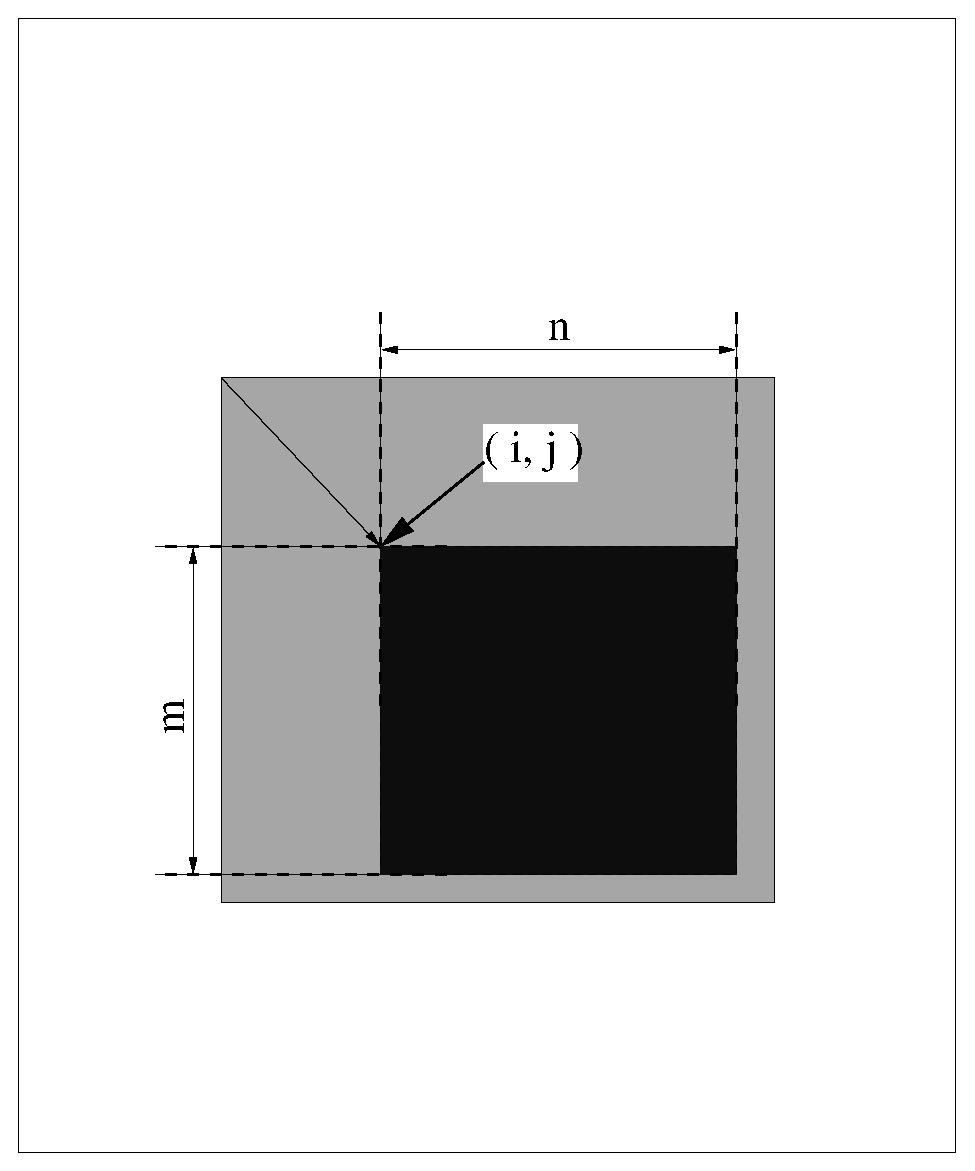
\includegraphics[height=2.5in,width=2.5in]{figures/matsubview.eps} 
&
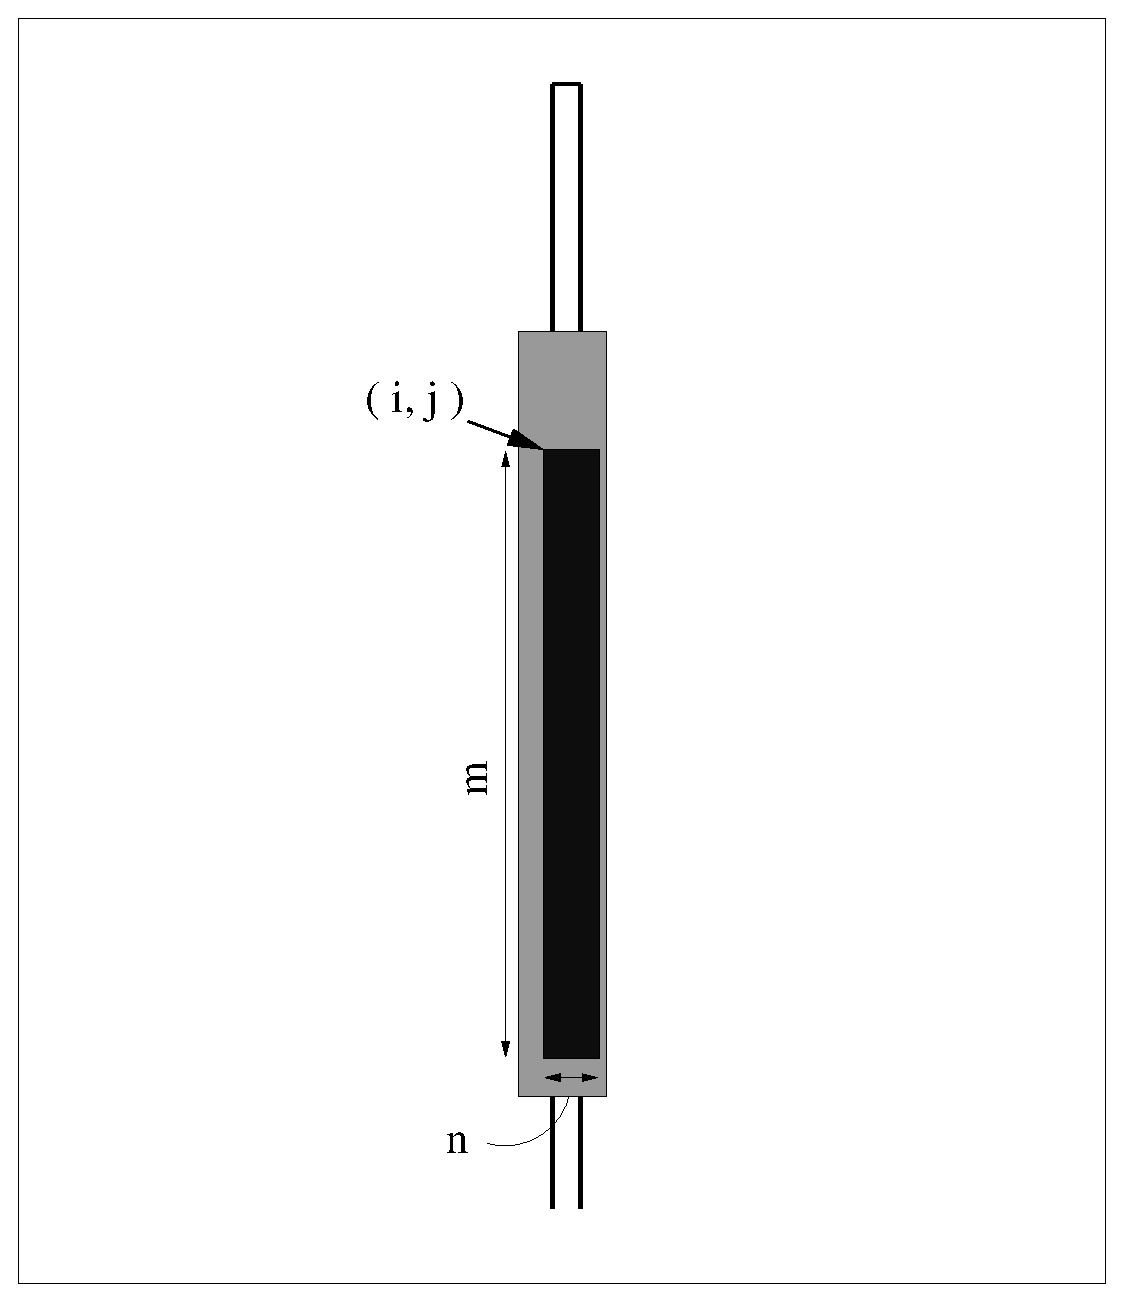
\includegraphics[height=2.5in,width=2.5in]{figures/mvectsubview.eps}
\\
\end{tabular}
\end{center}
\caption{
{\bf Left:}
A sub-matrix of a given matrix, starting at element
$ (i,j)$.
The row dimension of the sub-matrix is given by {\tt m}
and column dimension by {\tt n}.
{\bf Right:} 
A sub-multivector of a given multivector, starting at element
$ (i,j)$.
The row dimension of the sub-matrix is given by {\tt m}
and column dimension by {\tt n}.
}
\label{fig:views}
\end{figure}


The following illustrates a basic partitioning of a matrix
\renewcommand{\partitionings}{
$ 
A \rightarrow \FlaTwoByTwo{ A_{TL} }{ A_{TR} }
                          { A_{BL} }{ A_{BR} }
$
}
\renewcommand{\partitionsizes}{
$ A_{TL} $ is $ k \times k $
}
\begin{quote}
\WSpartition
\end{quote}
Given a descriptor {\tt A} of a matrix $ A $,
the following call creates descriptors of the four quadrants
\begin{FlaSpec}
\begin{verbatim}
PLA_Part_2x2( PLA_Obj A, PLA_Obj *ATL, PLA_Obj *ATR,
                         PLA_Obj *ABL, PLA_Obj *ABR,
              int mb, int nb, PLA_Quadrant quadrant )
\end{verbatim}
\purpose{Partition matrix {\tt A} into four quadrants
where the quadrant indicated by 
{\tt quadrant} is $ {\tt mb} \times {\tt nb} $.}
\parameter{\tt A}{matrix to be partitioned}
\parameter{\tt mb, nb}{row and column dimensions of quadrant indicated by {\tt quadrant}}
\parameter{\tt quadrant}{quadrant for which dimensions are given in {\tt mb}
and {\tt nb}}
\parameter{ATL-ABR}{views of TL, TR, BL, and BR quadrants}
\end{FlaSpec}
Here {\tt quadrant} can take on the
values {\tt PLA\_TL},
{\tt PLA\_TR},
{\tt PLA\_BL},
 and {\tt PLA\_BR}
to indicate that {\tt mb} and {\tt nb}
specify the dimensions of 
the \underline{T}op-\underline{L}eft,
\underline{T}op-\underline{R}ight,
\underline{B}ottom-\underline{L}eft, or
\underline{B}ottom-\underline{R}ight 
quadrant, respectively.
Thus, the algorithm fragment on the left
is translated into the code on the right
\renewcommand{\partitionings}{
$ 
A \rightarrow \FlaTwoByTwo{ A_{TL} }{ A_{TR} }
                          { A_{BL} }{ A_{BR} }
$
}
\renewcommand{\partitionsizes}{
$ A_{TL} $ is $ m_b \times n_b $
}
\begin{center}
\begin{tabular}{p{2.2in} | p{2.5in}}
\begin{minipage}{1.9in}
\WSpartition
\end{minipage}
&
\begin{minipage}{2.5in}
\footnotesize
\begin{verbatim}
PLA_Part_2x2( A,   &ATL, /**/ &ATR,
                /* *************** */
                   &ABL, /**/ &ABR,
              mb, nb, PLA_TL );
\end{verbatim}
\end{minipage}
\end{tabular}
\end{center}
where parameters {\tt mb} and {\tt nb} have values $ m_b $ and $ n_b $,
respectively.

An operation is needed that 
takes a $ 2 \times 2 $ partitioning of a given 
matrix $ A $ and repartitions this matrix into a 
$ 3 \times 3 $ partitioning so that submatrices 
that need to be updated and/or used for computation can be identified.
To support this operation, we introduce the call
\begin{FlaSpec}
\begin{verbatim}
PLA_Repart_from_2x2_to_3x3
\end{verbatim}
{\footnotesize
\begin{verbatim}
      ( PLA_Obj ATL, PLA_Obj ATR,   PLA_Obj *A00, PLA_Obj *A01, PLA_Obj *A02,
                                    PLA_Obj *A10, PLA_Obj *A11, PLA_Obj *A12,
        PLA_Obj ABL, PLA_Obj ABR,   PLA_Obj *A20, PLA_Obj *A21, PLA_Obj *A22,
        int mb, int nb, PLA_Quadrant quadrant )
\end{verbatim}
}
\purpose{Repartition a $ 2 \times 2 $ partitioning of matrix {\tt A} into 
a $ 3 \times 3 $ partitioning where $ {\tt mb} \times {\tt nb} $
submatrix {\tt A11} is split from 
the quadrant indicated by {\tt quadrant}.}
\parameter{\tt ATL-ABR}{views of TL, TR, BL, and BR quadrants}
\parameter{\tt mb, nb}{row and column dimensions of $ A_{11} $}
\parameter{\tt quadrant}{quadrant from which $ A_{11} $ is partitioned}
\parameter{A00-A22}{views of $ A_{00} $--$ A_{22} $}
\end{FlaSpec}
Here {\tt quadrant} can again take on the
values {\tt PLA\_TL}, {\tt PLA\_TR},
{\tt PLA\_BL}, and {\tt PLA\_{BR}}
to indicate that {\tt mb} and {\tt nb}
submatrix {\tt A11} is split from 
submatrix {\tt ATL}, {\tt ATR},
{\tt ABL}, or {\tt ABR}, respectively.

Thus,
\renewcommand{\blocksize}{1}
\renewcommand{\repartitionings}{
$ \FlaTwoByTwo{ A_{TL} }{ A_{TR} }
            { A_{BL} }{ L_{BR} }
\rightarrow
\FlaThreeByThreeBR{ A_{00} }{ A_{01} }{ A_{02} }
                { A_{10} }{ A_{11} }{ A_{12} }
                { A_{20} }{ A_{21} }{ A_{22} }
$
}
\renewcommand{\repartitionsizes}{
$ A_{11} $ is $ m_b \times n_b $
}
\begin{quote}
\WSrepartition
\end{quote} 
is captured in the code
\begin{quote}
\footnotesize
\begin{verbatim}
PLA_Repart_from_2x2_to_3x3( ATL, ATR,   &A00, /**/ &A01, &A02,
                                     /* ********************* */
                                        &A10, /**/ &A11, &A12,
                            ABL, ABR,   &A20, /**/ &A21, &A22,
                            mb, nb, PLA_BR );
\end{verbatim}
\end{quote}
where parameters {\tt mb} and {\tt nb} have values $ m_b $ and $ n_b $,
respectively.

Once the contents of the corresponding views have been updated, 
the descriptions of $ A_{TL} $, $ A_{TR} $, 
$ A_{BL} $, and $ A_{BR} $ must be updated 
to reflect that progress is being made in terms of the regions
identified by the double-lines.
Moving the double-lines is achieved by a call to
\begin{FlaSpec}
\begin{verbatim}
PLA_Cont_with_3x3_to_2x2
\end{verbatim}
{\footnotesize
\begin{verbatim}
      ( PLA_Obj *ATL, PLA_Obj *ATR,   PLA_Obj A00, PLA_Obj A01, PLA_Obj A02,
                                      PLA_Obj A10, PLA_Obj A11, PLA_Obj A12,
        PLA_Obj *ABL, PLA_Obj *ABR,   PLA_Obj A20, PLA_Obj A21, PLA_Obj A22,
        PLA_Quadrant quadrant )
\end{verbatim}
}
\purpose{
Update the $ 2 \times 2 $ partitioning of matrix {\tt A} by 
moving the boundaries so that {\tt A11} is added to 
the quadrant indicated by {\tt quadrant}.
}
\parameter{ATL-ABR}{views of TL, TR, BL, and BR quadrants}
\parameter{\tt A00-A22}{views of $ A_{00} $--$ A_{22} $}
\parameter{\tt quadrant}{quadrant to which $ A_{11} $ is to be added}
\end{FlaSpec}
Here the value of {\tt quadrant} 
({\tt PLA\_TL}, {\tt PLA\_TR},
{\tt PLA\_BL}, or {\tt PLA\_{BR}})
specifies the quadrant
submatrix {\tt A11} is to be added.

For example,
\renewcommand{\moveboundaries}{
$ \FlaTwoByTwo{ A_{TL} }{ A_{TR} }
            { A_{BL} }{ L_{BR} }
\leftarrow
\FlaThreeByThreeTL{ A_{00} }{ A_{01} }{ A_{02} }
                  { A_{10} }{ A_{11} }{ A_{12} }
                  { A_{20} }{ A_{21} }{ A_{22} }
$
}
\begin{quote}
\WSmoveboundary
\end{quote} 
translates to the code
\begin{quote}
\footnotesize
\begin{verbatim}
PLA_Cont_with_3x3_to_2x2( &ATL, &ATR,   A00, A01, /**/ A02,
                                        A10, A11, /**/ A12,
                                     /* ****************** */
                          &ABL, &ABR,   A20, A21, /**/ A22,
                          PLA_TL );
\end{verbatim}
\end{quote}

A matrix can also be partitioned horizontally into two submatrices
with the call
\begin{FlaSpec}
\begin{verbatim}
PLA_Part_2x1( PLA_Obj A, PLA_Obj *AT,
                         PLA_Obj *AB, 
              int mb, PLA_Side side )
\end{verbatim}
\purpose{Partition matrix {\tt A} into a top and bottom side
where the side indicated by 
{\tt side} has $ {\tt mb} $ rows.}
\parameter{\tt A}{matrix to be partitioned}
\parameter{\tt mb}{row dimension of side indicated by {\tt side}}
\parameter{\tt side}{side for which row dimension is given}
\parameter{AT, AB}{view of Top and Bottom part}
\end{FlaSpec}
Here {\tt side} can take on the
values {\tt PLA\_TOP} or  {\tt PLA\_BOTTOM}
to indicate that {\tt mb} indicates 
the row dimension of {\tt AT} or {\tt AB},
respectively.

Given that matrix $ A $ is already partitioned horizontally
it can be repartitioned into three submatrices with the call
\begin{FlaSpec}
\begin{verbatim}
PLA_Repart_from_2x1_to_3x1( PLA_Obj AT,   PLA_Obj *A0, 
                                          PLA_Obj *A1, 
                            PLA_Obj AB,   PLA_Obj *A2, 
                            int mb, PLA_Side side )
\end{verbatim}
\purpose{Repartition a $ 2 \times 1 $ partitioning of matrix {\tt A} into 
a $ 3 \times 1 $ partitioning where 
submatrix {\tt A1} with $ {\tt mb} $ rows is split from 
the side indicated by {\tt side}.}
\parameter{\tt AT, AB}{views of Top and Bottom sides}
\parameter{\tt mb}{row dimension of $ A_{1} $}
\parameter{\tt side}{side from which $ A_{1} $ is partitioned}
\parameter{A0-A2}{views of $ A_{0} $--$ A_{2} $}
\end{FlaSpec}
Here {\tt side} can take on the
values {\tt PLA\_TOP} or  {\tt PLA\_BOTTOM}
to indicate that {\tt mb} submatrix {\tt A1} 
is partitioned from {\tt AT} or {\tt AB},
respectively.

Given a $ 3 \times 1 $ partitioning of a given matrix $ A $,
the middle submatrix can be appended to either the first or
last submatrix with the call
\begin{FlaSpec}
\begin{verbatim}
PLA_Cont_with_3x1_to_2x1( PLA_Obj *AT,   PLA_Obj A0, 
                                         PLA_Obj A1, 
                          PLA_Obj *AB,   PLA_Obj A2, 
                          PLA_Side side )
\end{verbatim}
\purpose{
Update the $ 2 \times 1 $ partitioning of matrix {\tt A} by 
moving the boundaries so that {\tt A1} is added to 
the side indicated by {\tt side}.}
\parameter{AT, AB}{views of Top and Bottom sides}
\parameter{\tt A0-A2}{views of $ A_{0} $--$ A_{2} $}
\parameter{\tt side}{side from which $ A_{1} $ is partitioned}
\end{FlaSpec}

Finally, a matrix can be partitioned and repartitioned
vertically with the calls
\begin{FlaSpec}
\begin{verbatim}
PLA_Part_1x2( PLA_Obj A,   PLA_Obj *AL, PLA_Obj *AR, 
              int nb, PLA_Side side )
\end{verbatim}
\purpose{Partition matrix {\tt A} into a left and right side
where the side indicated by 
{\tt side} has $ {\tt nb} $ columns.}
\parameter{\tt A}{matrix to be partitioned}
\parameter{\tt nb}{column dimension of side indicated by {\tt side}}
\parameter{\tt side}{side for which column dimension is given}
\parameter{AL, AR}{view of Left and Right part}
\end{FlaSpec}
and
\begin{FlaSpec}
\begin{verbatim}
PLA_Repart_from_1x2_to_1x3( PLA_Obj  AL,              PLA_Obj  AR,     
                            PLA_Obj *A0, PLA_Obj *A1, PLA_Obj *A2, 
                            int nb, PLA_Side side )
\end{verbatim}
\purpose{Repartition a $ 1 \times 2 $ partitioning of matrix {\tt A} into 
a $ 1 \times 3 $ partitioning where 
submatrix {\tt A1} with $ {\tt nb} $ columns is split from 
the side indicated by {\tt side}.}
\parameter{\tt AL, AR}{views of Left and Right sides}
\parameter{A0-A2}{views of $ A_{0} $--$ A_{2} $}
\parameter{\tt nb}{column dimension of $ A_{1} $}
\parameter{\tt side}{side from which $ A_{1} $ is partitioned}
\end{FlaSpec}
Here {\tt side} can take on the
values {\tt PLA\_LEFT} or  {\tt PLA\_RIGHT}.
Adding the middle submatrix to the first or last is 
now accomplished by a call to
\begin{FlaSpec}
\begin{verbatim}
PLA_Cont_with_1x3_to_1x2( PLA_Obj *AL,             PLA_Obj *AR,  
                          PLA_Obj  A0, PLA_Obj A1, PLA_Obj  A2, 
                          PLA_Side side )
\end{verbatim}
\purpose{Update the $ 1 \times 2 $ partitioning of matrix {\tt A} by 
moving the boundaries so that {\tt A1} is added to 
the side indicated by {\tt side}.}
\parameter{AL, AR}{views of Left and Right sides}
\parameter{\tt side}{side to which $ A_{1} $ is added}
\parameter{\tt A0-A2}{views of $ A_{0} $--$ A_{2} $}
\end{FlaSpec}


\subsection{Determining where to split}

For performance reasons, it is often important to
partition the linear algebra object on a template block
boundary (e.g. when it is
necessary to guarantee that a specific sub-matrix or
sub-vector exists entirely on one node).
To determine the size that can be split on
a given side of an object, we provide the call
\begin{FlaSpec}
\begin{verbatim}
int PLA_Obj_split_size( PLA_Obj A, PLA_Side side )
\end{verbatim}
\purpose{Compute size of split to next block boundary.}
\parameter{\tt A}{object being referenced by view}
\parameter{\tt side}{side to find block boundary}
\parameter{return}{length to the next template {\em sub-block} split}
\end{FlaSpec}
This call returns the size to the block boundary 
towards the center of the view on the specified side.
Here {\tt side} can take the values of 
\begin{center}
{\tt PLA\_TOP}, {\tt PLA\_BOTTOM}, {\tt PLA\_LEFT}, {\tt PLA\_RIGHT},
{\tt PLA\_TL}, {\tt PLA\_TR}, {\tt PLA\_BL}, and {\tt PLA\_BR}.
\end{center}
If the quadrants are selected, the minimum value to the 
block boundary to the horizontal and vertical edges is returned.



\section{Example: Matrix-Vector Multiplication}

We now give an example of how to use the calls introduced so
far to write a simple driver routine that calls a routine
that performs the matrix-vector multiplication $ y = A x $.
\begin{figure}[htp]
\center
\fbox{
\hspace*{.1in}
    \begin{minipage}{4.6in}
    \footnotesize
    \listinginput[1]{1}{examples/mv_mult.c}
  \end{minipage}
}
\caption{A simple driver for matrix-vector multiplication.}
\label{code:mv_mult}
\end{figure}

In Fig.~\ref{code:mv_mult} we give the driver routine.
\begin{itemize}
\item{\bf line 1--2:}
plapack program files start by including the 
{\tt mpi.h} and {\tt PLA.h} header files.
\item
{\bf line 10--11:}
The MPI communicator used to create the template is declared
as the global MPI communicator {\tt MPI\_COMM\_WORLD}.
\item
{\bf line 13--14:}
The template {\tt templ} is declared, but 
the predefined, default template {\tt PLA\_TEMP\_WORLD} could also be used.
\item
{\bf line 16--17:}
The objects {\tt A}, {\tt x}, and {\tt y},
which will hold matrix $ A $ and vectors $ x $ and $ y $, 
are all declared to be of type {\tt PLA\_Obj}.
\item
{\bf line 19--20:}
Before any calls to plapack routines can be
made, the environment must be initialized by
a call to {\tt MPI\_Init} first and then {\tt PLA\_Init}.
\item
{\bf line 22--37:}
In our example, the user inputs the row 
and column dimension of matrix $ A $ 
along with dimensions describing the template.
These values are distributed to each node used 
the plapack environment with {\tt MPI\_Bcast}.
\item
{\bf line 39--41:}
The template is created where the
inducing column and row vectors are set
to the recommended values of row-major and column-major, respectively.
\item
{\bf line 43--53:}
Descriptors are created for $ A $, $ x $, and $ y $.
\item
{\bf line 55:}
The routine {\tt fill}, described in Fig.~\ref{code:fill}, 
is used to fill $ A $, $ x $, and $ y $ with values.
\item
{\bf line 57:}
Compute $ y = A x $ using {\tt PLA\_Gemv}.
\item
{\bf line 59--60:}
Free the created objects.
\item
{\bf line 62--63:}
Finalize the MPI and plapack environments.
\end{itemize}

A sample routine for filling {\tt A}, {\tt x} and {\tt y}
with data is given in Fig.~\ref{code:fill}.  
{\tt PLA\_Gemv} is general matrix-vector multiply, which
performs internal communication and calls an internal
subroutine to perform local computation on each node and is described
in Ch.~\ref{chapter:blas}.

The routine in Fig.~\ref{code:fill} contains two nested loops that traverse 
any object in column-major order using views into that object.  
Each element in the
object {\tt A} has encoded its row and column dimensions
and the rank of the processor where it resides.
This routine is not the preferred method for filling matrices,
which is presented in Ch.~\ref{chapter:api}.
\begin{figure}[htp]
\center
\fbox{
\hspace*{.1in}
    \begin{minipage}{4.6in}
    \footnotesize
    \listinginput[1]{1}{examples/fill.c}
  \end{minipage}
}
\caption{A simple routine for filling objects.}
\label{code:fill}
\end{figure}


\section{Return values}

Unless otherwise specified, all plapack calls have a return type of 
{\tt PLA\_Error} which represents an error code.  
A return value of {\tt PLA\_SUCCESS}(= 0)
indicates the called routines completely successfully, otherwise
{\tt PLA\_FAILURE}($\neq$ 0) is returned.
